% Capitolul 0: Fundamente ale Analizei Seriilor de Timp
% Prezentare academică de calitate Harvard
% Program de licență, Academia de Studii Economice din București

\documentclass[9pt, aspectratio=169, t]{beamer}

% Asigură încadrarea conținutului pe diapozitive
\setbeamersize{text margin left=8mm, text margin right=8mm}

%=============================================================================
% CONFIGURARE TEMĂ ȘI STIL
%=============================================================================
\usetheme{default}
% Utilizăm tema implicită pentru control curat al antetului/subsolului

% Paletă de Culori (potrivită cu PDF-ul Redispatch)
\definecolor{MainBlue}{RGB}{26, 58, 110}
\definecolor{AccentBlue}{RGB}{26, 58, 110}
\definecolor{IDAred}{RGB}{205, 0, 0}
\definecolor{DarkGray}{RGB}{51, 51, 51}
\definecolor{MediumGray}{RGB}{128, 128, 128}
\definecolor{LightGray}{RGB}{248, 248, 248}
\definecolor{VeryLightGray}{RGB}{235, 235, 235}
\definecolor{KeynoteGray}{RGB}{218, 218, 218}
\definecolor{SectionGray}{RGB}{120, 120, 120}
\definecolor{FooterGray}{RGB}{100, 100, 100}
\definecolor{Crimson}{RGB}{220, 53, 69}
\definecolor{Forest}{RGB}{46, 125, 50}
\definecolor{Amber}{RGB}{181, 133, 63}
\definecolor{Orange}{RGB}{230, 126, 34}
\definecolor{Purple}{RGB}{142, 68, 173}

% Fundal gradient (gradient Keynote exact 315°: alb la RGB 218,218,218)
\setbeamertemplate{background}{%
    \begin{tikzpicture}[remember picture, overlay]
        \shade[shading=axis, shading angle=315,
        top color=white, bottom color=KeynoteGray]
        (current page.south west) rectangle (current page.north east);
    \end{tikzpicture}%
}
% Culoare solidă de rezervă pentru compatibilitate
\setbeamercolor{background canvas}{bg=}

\setbeamercolor{palette primary}{bg=MainBlue, fg=white}
\setbeamercolor{palette secondary}{bg=MainBlue!85, fg=white}
\setbeamercolor{palette tertiary}{bg=MainBlue!70, fg=white}
\setbeamercolor{structure}{fg=MainBlue}
\setbeamercolor{title}{fg=IDAred}
\setbeamercolor{frametitle}{fg=IDAred, bg=}
\setbeamercolor{block title}{bg=MainBlue, fg=white}
\setbeamercolor{block body}{bg=VeryLightGray, fg=DarkGray}
\setbeamercolor{block title alerted}{bg=Crimson, fg=white}
\setbeamercolor{block body alerted}{bg=Crimson!8, fg=DarkGray}
\setbeamercolor{block title example}{bg=Forest, fg=white}
\setbeamercolor{block body example}{bg=Forest!8, fg=DarkGray}
\setbeamercolor{item}{fg=MainBlue}

% Culori subsol (suprascriu albastrul temei Madrid)
\setbeamercolor{author in head/foot}{fg=FooterGray, bg=}
\setbeamercolor{title in head/foot}{fg=FooterGray, bg=}
\setbeamercolor{date in head/foot}{fg=FooterGray, bg=}
\setbeamercolor{section in head/foot}{fg=FooterGray, bg=}
\setbeamercolor{subsection in head/foot}{fg=FooterGray, bg=}

% Stiluri marcatori (se aplică peste tot inclusiv în blocuri)
\setbeamertemplate{itemize item}{\color{MainBlue}$\boxdot$}
\setbeamertemplate{itemize subitem}{\color{MainBlue}$\blacktriangleright$}
\setbeamertemplate{itemize subsubitem}{\color{MainBlue}\tiny$\bullet$}
\setbeamertemplate{itemize/enumerate body begin}{\normalsize}
\setbeamertemplate{itemize/enumerate subbody begin}{\normalsize}

% Item spacing - compact style
\setlength{\leftmargini}{10pt}       % Level 1: minimal indent
\setlength{\leftmarginii}{10pt}      % Level 2: minimal additional indent
% Compact list spacing (zero extra space before/after lists in blocks)
\makeatletter
\def\@listi{\leftmargin\leftmargini \topsep 0pt \parsep 0pt \itemsep 0pt}
\def\@listii{\leftmargin\leftmarginii \topsep 0pt \parsep 0pt \itemsep 0pt}
\makeatother

\setbeamertemplate{navigation symbols}{}

%=============================================================================
% CUSTOM HEADLINE
%=============================================================================
\setbeamertemplate{headline}{%
    \vskip10pt%
    \hbox to \paperwidth{%
        \hskip0.5cm%
        {\small\color{FooterGray}\renewcommand{\hyperlink}[2]{##2}\insertsectionhead}%
        \hfill%
        \textcolor{FooterGray}{\small\insertframenumber}%
        \hskip0.5cm%
    }%
    \vskip4pt%
    {\color{FooterGray}\hrule height 0.4pt}%
}

%=============================================================================
% CUSTOM FOOTER
%=============================================================================
\usepackage{fontawesome5}

\setbeamertemplate{footline}{%
    {\color{FooterGray}\hrule height 0.4pt}%
    \vskip4pt%
    \hbox to \paperwidth{%
        \hskip0.5cm%
        \textcolor{FooterGray}{\small Analiza și Prognoza Seriilor de Timp}%
        \hfill%
        \raisebox{-0.1em}{%
            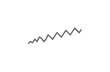
\begin{tikzpicture}[x=0.08em, y=0.08em, line width=0.4pt]
                \draw[FooterGray] (0,3) -- (1,4) -- (2,3.5) -- (3,5) -- (4,4) -- (5,6) -- (6,5.5) -- (7,4) -- (8,5) -- (9,7) -- (10,6) -- (11,5) -- (12,6.5) -- (13,8) -- (14,7) -- (15,6) -- (16,7.5) -- (17,9) -- (18,8) -- (19,7) -- (20,8.5) -- (21,10) -- (22,9) -- (23,8) -- (24,9.5);
            \end{tikzpicture}%
        }%
        \hskip0.5cm%
    }%
    \vskip6pt%
}

%=============================================================================
% PACHETE
%=============================================================================
\usepackage[utf8]{inputenc}
\usepackage[T1]{fontenc}
\usepackage{amsmath, amssymb, amsthm}
\usepackage{mathtools}
\usepackage{bm}
\usepackage{tikz}
\usetikzlibrary{arrows.meta, positioning, shapes, calc, decorations.pathreplacing, shadings}
\usepackage{booktabs}
\usepackage{multirow}
\usepackage{array}
\usepackage{graphicx}
\usepackage{hyperref}
\usepackage{colortbl}
\hypersetup{colorlinks=true, linkcolor=MainBlue, urlcolor=MainBlue}
\graphicspath{{../../logos/}{../../charts/}}
\hfuzz=2pt  % Suppress tiny overfull warnings (<2pt)
\vfuzz=10pt  % Suppress vertical overfull warnings (<10pt)

%=============================================================================
% COMANDA QUANTLET
%=============================================================================
\newcommand{\quantlet}[2]{%
    \hfill\href{#2}{%
        \raisebox{-0.15em}{\includegraphics[height=0.7em]{ql_logo.png}}%
        \textcolor{MainBlue}{\tiny\ #1}%
    }%
}

%=============================================================================
% PAGINĂ TITLU PERSONALIZATĂ
%=============================================================================
\defbeamertemplate*{title page}{hybrid}[1][]
{
    \vspace{0.2cm}
    % Logos row - top header (with clickable links)
    \begin{center}
        \href{https://www.ase.ro}{\includegraphics[height=1.0cm]{ase_logo.png}}\hspace{0.3cm}%
        \href{https://theida.net}{\includegraphics[height=1.0cm]{ida_logo.png}}\hspace{0.3cm}%
        \href{https://blockchain-research-center.com}{\includegraphics[height=1.0cm]{brc_logo.png}}\hspace{0.3cm}%
        \href{https://www.ai4efin.ase.ro}{\includegraphics[height=1.0cm]{ai4efin_logo.png}}\hspace{0.3cm}%
        \href{https://ipe.ro/new}{\includegraphics[height=1.0cm]{acad_logo.png}}\hspace{0.3cm}%
        \href{https://www.digital-finance-msca.com}{\includegraphics[height=1.0cm]{msca_logo.png}}%
    \end{center}

    \vspace{0.6cm}

    % Main title with Q logos on sides (with clickable links)
    \begin{center}
        \begin{minipage}{0.1\textwidth}
            \centering
            \href{https://quantlet.com}{\includegraphics[height=1.1cm]{ql_logo.png}}
        \end{minipage}%
        \begin{minipage}{0.78\textwidth}
            \centering
            {\LARGE\bfseries\usebeamercolor[fg]{title}\inserttitle}

            \vspace{0.3cm}

            {\usebeamerfont{subtitle}\usebeamercolor[fg]{title}\insertsubtitle}
        \end{minipage}%
        \begin{minipage}{0.1\textwidth}
            \centering
            \href{https://quantinar.com}{\includegraphics[height=1.1cm]{qr_logo.png}}
        \end{minipage}
    \end{center}

    \vspace{0.6cm}

    % Authors (left aligned)
    \hspace{0.5cm}{\usebeamerfont{author}\insertauthor}

    \vspace{0.3cm}

    % Institute/Affiliations (left aligned)
    \hspace{0.5cm}\begin{minipage}[t]{0.9\textwidth}
        \raggedright\small\insertinstitute
    \end{minipage}
}

%=============================================================================
% CENTRED MINIPAGE (fara spatiu vertical suplimentar)
%=============================================================================
\newenvironment{cminipage}[1]{%
    \par\noindent\hfill\begin{minipage}{#1}\ignorespaces
}{%
    \end{minipage}\hfill\null\par
}

%=============================================================================
% MEDII PENTRU TEOREME
%=============================================================================
\theoremstyle{definition}
\setbeamertemplate{theorems}[numbered]
\newtheorem{defn}{Definiție}
\newtheorem{thm}{Teoremă}
\newtheorem{prop}{Propoziție}
\newtheorem{rmk}{Observație}

%=============================================================================
% COMENZI PERSONALIZATE
%=============================================================================
\newcommand{\E}{\mathbb{E}}
\newcommand{\Var}{\text{Var}}
\newcommand{\Cov}{\text{Cov}}
\newcommand{\Corr}{\text{Corr}}
\newcommand{\R}{\mathbb{R}}
\newcommand{\N}{\mathbb{N}}
\newcommand{\Z}{\mathbb{Z}}
\newcommand{\B}{\mathbf{B}}
\newcommand{\imark}{\textcolor{MainBlue}{\textbullet}}
\newcommand{\RMSE}{\text{RMSE}}
\newcommand{\MAE}{\text{MAE}}
\newcommand{\MAPE}{\text{MAPE}}

%=============================================================================
% INFORMAȚII TITLU
%=============================================================================
\title[Analiza Seriilor de Timp]{Analiza și Prognoza Seriilor de Timp}
\subtitle{Capitolul 0: Fundamente}
\author[D.T. Pele]{Daniel Traian PELE}
\institute{Academia de Studii Economice din București\\
IDA Institute Digital Assets\\
Blockchain Research Center\\
AI4EFin Artificial Intelligence for Energy Finance\\
Academia Română, Institutul de Prognoză Economică\\
MSCA Digital Finance}
\date{}

\begin{document}

% Title page (no header/footer)
{
\setbeamertemplate{headline}{}
\setbeamertemplate{footline}{}
\begin{frame}
    \titlepage
\end{frame}
}

%=============================================================================
% OBIECTIVE DE ÎNVĂȚARE
%=============================================================================
\begin{frame}{Obiective de Învățare}
    \textbf{\large La sfârșitul acestui capitol, veți putea să:}
    \vspace{0.15cm}
    \begin{enumerate}
        \item[\textcolor{MainBlue}{\textbf{1.}}] \textbf{Definiți} seriile de timp și să le distingeți de datele transversale și de panel
        \vspace{0.08cm}
        \item[\textcolor{MainBlue}{\textbf{2.}}] \textbf{Descompuneți} seriile de timp în componente de trend-ciclu, sezonalitate și reziduuri
        \vspace{0.08cm}
        \item[\textcolor{MainBlue}{\textbf{3.}}] \textbf{Aplicați} metodele de netezire exponențială (SES, Holt, Holt-Winters, ETS)
        \vspace{0.08cm}
        \item[\textcolor{MainBlue}{\textbf{4.}}] \textbf{Evaluați} prognozele folosind MAE, RMSE, MAPE, sMAPE
        \vspace{0.08cm}
        \item[\textcolor{MainBlue}{\textbf{5.}}] \textbf{Implementați} separarea train/validare/test și validarea încrucișată
        \vspace{0.08cm}
        \item[\textcolor{MainBlue}{\textbf{6.}}] \textbf{Modelați} sezonalitatea folosind variabile dummy sau termeni Fourier
        \vspace{0.08cm}
        \item[\textcolor{MainBlue}{\textbf{7.}}] \textbf{Eliminați} trendul și sezonalitatea prin metode adecvate
        \vspace{0.08cm}
        \item[\textcolor{MainBlue}{\textbf{8.}}] \textbf{Distingeți} între trendurile deterministe și stochastice
    \end{enumerate}
\end{frame}

%=============================================================================
% CUPRINS
%=============================================================================
\begin{frame}{Structura Capitolului}
    \setbeamertemplate{section in toc}{\color{MainBlue}$\boxdot$~\inserttocsection}
    \tableofcontents
\end{frame}

%=============================================================================
% MOTIVAȚIE
%=============================================================================
\section{Motivație}

\begin{frame}{Seriile de Timp Sunt Pretutindeni}
    \vspace{-0.3cm}
    \begin{center}
        \includegraphics[width=0.95\textwidth, height=0.60\textheight, keepaspectratio]{ch1_motivation_everywhere.png}
    \end{center}
    \vspace{-0.2cm}
    {\footnotesize
    \begin{itemize}
        \item \textbf{Finanțe}: Prețuri acțiuni, cursuri valutare, volume tranzacționate
        \item \textbf{Economie}: PIB, șomaj, rate ale inflației
        \item \textbf{Business}: Vânzări, trafic website, cererea clienților
        \item \textbf{Știință}: Temperatură, niveluri de poluare, semne vitale pacienți
    \end{itemize}
    }\quantlet{TSA\_ch1\_motivation}{https://github.com/QuantLet/TSA/tree/main/TSA_ch1/TSA_ch1_motivation}
\end{frame}

\begin{frame}{De Ce Studiem Seriile de Timp?}
    \vspace{-0.2cm}
    \begin{center}
        \includegraphics[width=0.95\textwidth, height=0.62\textheight, keepaspectratio]{ch1_motivation_forecast.png}
    \end{center}
    \vspace{-0.3cm}
    {\footnotesize
    \begin{alertblock}{Obiectiv Principal: Prognoza}
        Folosim tiparele istorice pentru a prezice valori viitoare --- esențial pentru planificarea afacerilor, managementul riscului și deciziile de politică.
    \end{alertblock}
    }\quantlet{TSA\_ch1\_forecast}{https://github.com/QuantLet/TSA/tree/main/TSA_ch1/TSA_ch1_forecast}
\end{frame}

\begin{frame}{Înțelegerea Structurii Seriilor de Timp}
    \vspace{-0.2cm}
    \begin{center}
        \includegraphics[width=0.92\textwidth, height=0.62\textheight, keepaspectratio]{ch1_motivation_components.png}
    \end{center}
    \vspace{-0.3cm}
    {\footnotesize
    \begin{exampleblock}{Descompunere}
        Orice serie de timp poate fi descompusă în componente interpretabile: trend-ciclu, sezonalitate și zgomot.
    \end{exampleblock}
    }\quantlet{TSA\_ch1\_components}{https://github.com/QuantLet/TSA/tree/main/TSA_ch1/TSA_ch1_components}
\end{frame}

%=============================================================================
% SECȚIUNEA 1: CE ESTE O SERIE DE TIMP
%=============================================================================
\section{Ce Este o Serie de Timp?}

\begin{frame}{Definiția unei Serii de Timp}
    \begin{defn}[Serie de Timp]
        O \textbf{serie de timp} este o secvență de observații $\{X_t\}$ indexate după timp:
        \[
            \{X_t : t \in \mathcal{T}\}
        \]
        unde $\mathcal{T}$ este o mulțime de indici reprezentând momente de timp.
    \end{defn}

    \vspace{0.2cm}

    \begin{columns}[T]
        \column{0.5\textwidth}
        \begin{block}{Caracteristici Cheie}
            \begin{itemize}
                \item \textbf{Ordonate}: Ordine temporală naturală
                \item \textbf{Dependente}: Observațiile consecutive sunt corelate
                \item \textbf{Discrete/Continue}: $t = 1, 2, 3, \ldots$
            \end{itemize}
        \end{block}

        \column{0.5\textwidth}
        \begin{exampleblock}{Notație}
            \begin{itemize}
                \item $X_t$ = observația la momentul $t$
                \item $\{X_t\}_{t=1}^{T}$ = serie cu $T$ observații
            \end{itemize}
        \end{exampleblock}
    \end{columns}
\end{frame}

\begin{frame}{Serie de Timp: Ilustrație Vizuală}
    \begin{columns}[T]
        \column{0.35\textwidth}
        \begin{exampleblock}{Interpretare}
            Fiecare punct $X_t$ reprezintă o observație la momentul $t$. Secvența este ordonată și observațiile consecutive sunt de obicei corelate.
        \end{exampleblock}
        \vspace{0.3cm}
        \quantlet{TSA\_ch1\_def\_timeseries}{https://github.com/QuantLet/TSA/tree/main/TSA_ch1/TSA_ch1_def_timeseries}
        \column{0.63\textwidth}
        \vspace{-0.3cm}
        \begin{center}
            \includegraphics[width=\textwidth, height=0.78\textheight, keepaspectratio]{ch1_def_timeseries.pdf}
        \end{center}
    \end{columns}
\end{frame}

\begin{frame}{Tipare Comune în Seriile de Timp}
    \begin{columns}[T]
        \column{0.38\textwidth}
        \begin{block}{Tipuri de Tipare}
            \begin{itemize}
                \item \textbf{Trend}: Creștere sau scădere pe termen lung
                \item \textbf{Sezonier}: Tipare periodice regulate
                \item \textbf{Ciclic}: Fluctuații pe termen mediu (2--10 ani)
                \item \textbf{Aleatoriu}: Fluctuații imprevizibile
            \end{itemize}
        \end{block}
        \column{0.60\textwidth}
        \vspace{-0.3cm}
        \begin{center}
            \includegraphics[width=\textwidth, height=0.75\textheight, keepaspectratio]{ch1_ts_patterns.pdf}
        \end{center}
    \end{columns}
    \quantlet{TSA\_ch1\_patterns}{https://github.com/QuantLet/TSA/tree/main/TSA_ch1/TSA_ch1_patterns}
\end{frame}

\begin{frame}{Serie de Timp: Definiție Vizuală}
    \begin{columns}[T]
        \column{0.35\textwidth}
        \begin{block}{Interpretare}
            Fiecare punct $X_t$ reprezintă o măsurătoare la momentul discret $t$. Ordinea temporală creează dependență între observații. Date: S\&P 500 (2024).
        \end{block}
        \vspace{0.3cm}
        \quantlet{TSA\_ch1\_definition}{https://github.com/QuantLet/TSA/tree/main/TSA_ch1/TSA_ch1_definition}
        \column{0.63\textwidth}
        \vspace{-0.3cm}
        \begin{center}
            \includegraphics[width=\textwidth, height=0.78\textheight, keepaspectratio]{timeseries_definition.pdf}
        \end{center}
    \end{columns}
\end{frame}

\begin{frame}{Tipuri de Date: Comparație}
    \begin{center}
        \includegraphics[width=0.95\textwidth, height=0.52\textheight, keepaspectratio]{data_types_comparison.png}
    \end{center}
    \vspace{-0.2cm}
    \begin{center}
    \small
    \begin{tabular}{lccc}
        \toprule
        \textbf{Tip de Date} & \textbf{Unități ($N$)} & \textbf{Timp ($T$)} & \textbf{Exemplu} \\
        \midrule
        Transversale & Multe & 1 & Sondaj pe 1000 gospodării \\
        Serie de timp & 1 & Multe & Prețuri zilnice S\&P 500 \\
        Panel & Multe & Multe & PIB-ul a 50 țări, 20 ani \\
        \bottomrule
    \end{tabular}
    \end{center}
    \quantlet{TSA\_ch1\_data\_types}{https://github.com/QuantLet/TSA/tree/main/TSA_ch1/TSA_ch1_data_types}
\end{frame}

\begin{frame}{Exemple de Date de Tip Serie de Timp}
    \begin{columns}[T]
        \column{0.35\textwidth}
        \begin{exampleblock}{Date Financiare Reale}
            Yahoo Finance (2019--2025), normalizate la baza 100. Observați tiparele diferite de volatilitate: Bitcoin cel mai volatil, Aurul cel mai stabil.
        \end{exampleblock}
        \vspace{0.3cm}
        \quantlet{TSA\_ch1\_examples}{https://github.com/QuantLet/TSA/tree/main/TSA_ch1/TSA_ch1_examples}
        \column{0.63\textwidth}
        \vspace{-0.3cm}
        \begin{center}
            \includegraphics[width=\textwidth, height=0.78\textheight, keepaspectratio]{multiple_assets.pdf}
        \end{center}
    \end{columns}
\end{frame}

%=============================================================================
% SECȚIUNEA 2: DESCOMPUNEREA SERIILOR DE TIMP
%=============================================================================
\section{Descompunerea Seriilor de Timp}

\begin{frame}{De Ce Descompunem o Serie de Timp?}
    \textbf{Descompunerea} separă o serie de timp în componente interpretabile:

    \vspace{0.15cm}

    \begin{columns}[T]
        \begin{column}{0.48\textwidth}
            \textbf{Obiective:}
            \begin{itemize}
                \item Înțelegerea tiparelor subiacente
                \item Eliminarea sezonalității pentru modelare
                \item Identificarea direcției trendului
                \item Izolarea fluctuațiilor neregulate
                \item Îmbunătățirea acurateții prognozei
            \end{itemize}
        \end{column}
        \begin{column}{0.48\textwidth}
            \textbf{Componente:}
            \begin{itemize}
                \item $T_t$ = \textbf{Trend-Ciclu}: Mișcare pe termen lung
                \item $S_t$ = \textbf{Sezonier}: Tipar periodic regulat
                \item $\varepsilon_t$ = \textbf{Reziduu}: Zgomot aleatoriu
            \end{itemize}
            {\footnotesize\textit{Notă: Componenta ciclică este de obicei absorbită în $T_t$}}
        \end{column}
    \end{columns}

    \vspace{0.2cm}

    \begin{block}{Modele Clasice de Descompunere}
        \begin{itemize}
            \item \textbf{Aditiv}: $X_t = T_t + S_t + \varepsilon_t$
            \item \textbf{Multiplicativ}: $X_t = T_t \times S_t \times \varepsilon_t$
        \end{itemize}
    \end{block}
\end{frame}

\begin{frame}{Descompunerea Seriilor de Timp: Exemplu Vizual}
    \vspace{-0.2cm}
    \begin{center}
        \includegraphics[width=0.95\textwidth, height=0.55\textheight, keepaspectratio]{ch1_decomposition.png}
    \end{center}
    \vspace{-0.2cm}
    \begin{exampleblock}{Interpretare}
        Descompunere aditivă: $Y = T + S + R$. Componentele sunt cele definite pe slide-ul anterior.
    \end{exampleblock}
    \quantlet{TSA\_ch1\_decomposition}{https://github.com/QuantLet/TSA/tree/main/TSA_ch1/TSA_ch1_decomposition}
\end{frame}

\begin{frame}{Componenta Ciclică}
    \vspace{-0.3cm}
    \begin{center}
        \includegraphics[width=0.95\textwidth, height=0.50\textheight, keepaspectratio]{ch1_cyclical_component.png}
    \end{center}
    \vspace{-0.2cm}
    {\small
    \begin{columns}[T]
        \column{0.48\textwidth}
        \begin{block}{Caracteristici}
            \begin{itemize}
                \item Fluctuații pe termen mediu (2--10 ani)
                \item Fără perioadă fixă (spre deosebire de sezonier)
                \item Reflectă expansiuni/recesiuni
            \end{itemize}
        \end{block}

        \column{0.48\textwidth}
        \begin{alertblock}{În Practică}
            \begin{itemize}
                \item Ciclul este adesea combinat cu trendul
                \item Dificil de identificat în serii scurte
                \item De obicei nu se modelează separat
            \end{itemize}
        \end{alertblock}
    \end{columns}
    }\quantlet{TSA\_ch1\_cyclical}{https://github.com/QuantLet/TSA/tree/main/TSA_ch1/TSA_ch1_cyclical}
\end{frame}

\begin{frame}{Modelul de Descompunere Aditivă}
    \begin{block}{Model}
        \vspace{-0.3cm}
        \begin{equation}
            X_t = T_t + S_t + \varepsilon_t
        \end{equation}
        \vspace{-0.3cm}
    \end{block}

    \vspace{0.2cm}

    \begin{columns}[T]
        \column{0.48\textwidth}
        \begin{exampleblock}{Când să Folosim}
            \begin{itemize}
                \item Fluctuațiile sezoniere sunt \textbf{constante} în timp
                \item Varianța seriei este \textbf{stabilă}
            \end{itemize}
        \end{exampleblock}

        \column{0.48\textwidth}
        \begin{block}{Proprietăți}
            \begin{itemize}
                \item $\E[\varepsilon_t] = 0$ (medie zero)
                \item $\sum_{j=1}^{s} S_j = 0$ (suma sezonală e zero)
                \item Unitățile $S_t$ sunt aceleași ca $X_t$
            \end{itemize}
        \end{block}
    \end{columns}
\end{frame}

\begin{frame}{Descompunere Aditivă: Vizualizare}
    \vspace{-0.2cm}
    \begin{center}
        \includegraphics[width=0.95\textwidth, height=0.62\textheight, keepaspectratio]{ts_components_synthetic.png}
    \end{center}
    \vspace{-0.3cm}
    \begin{block}{Interpretare}
        Original = Trend + Sezonier + Reziduu. Amplitudinea sezonieră rămâne constantă indiferent de nivel.
    \end{block}
    \quantlet{TSA\_ch0\_additive}{https://github.com/QuantLet/TSA/tree/main/TSA_ch0/TSA_ch0_additive}
\end{frame}

\begin{frame}{Modelul de Descompunere Multiplicativă}
    \begin{block}{Model}
        \vspace{-0.3cm}
        \begin{equation}
            X_t = T_t \times S_t \times \varepsilon_t
        \end{equation}
        \vspace{-0.3cm}
    \end{block}

    \vspace{0.2cm}

    \begin{columns}[T]
        \column{0.48\textwidth}
        \begin{exampleblock}{Când să Folosim}
            \begin{itemize}
                \item Fluctuațiile sezoniere \textbf{cresc} odată cu nivelul seriei
                \item Varianța \textbf{crește} în timp
            \end{itemize}
        \end{exampleblock}

        \column{0.48\textwidth}
        \begin{block}{Proprietăți}
            \begin{itemize}
                \item $\E[\varepsilon_t] = 1$ (centrat la 1)
                \item $\frac{1}{s}\sum S_j = 1$ (media e 1)
                \item $S_t$ este raport adimensional
            \end{itemize}
        \end{block}
    \end{columns}

    \vspace{0.2cm}

    \begin{alertblock}{Sfat}
        Transformarea logaritmică convertește modelul multiplicativ în aditiv: $\log X_t = \log T_t + \log S_t + \log \varepsilon_t$
    \end{alertblock}
\end{frame}

\begin{frame}{Descompunere Multiplicativă: Date Reale}
    \begin{columns}[T]
        \column{0.32\textwidth}
        \begin{exampleblock}{Exemplu}
            Clasicul set de date Box-Jenkins cu pasagerii companiilor aeriene (1949--1960). Amplitudinea sezonieră crește odată cu nivelul.
        \end{exampleblock}
        \vspace{0.3cm}
        \quantlet{TSA\_ch0\_multiplicative}{https://github.com/QuantLet/TSA/tree/main/TSA_ch0/TSA_ch0_multiplicative}
        \column{0.66\textwidth}
        \vspace{-0.3cm}
        \begin{center}
            \includegraphics[width=\textwidth, height=0.80\textheight, keepaspectratio]{airline_decomposition.pdf}
        \end{center}
    \end{columns}
\end{frame}

% Slide removed: "Aditivă vs Multiplicativă: Comparație" — redundant with individual model slides (17, 19)

\begin{frame}{Estimarea Trendului: Media Mobilă}
    \begin{defn}[Media Mobilă Centrată]
        \textbf{Media mobilă centrată} de ordin $2q+1$ este:
        \vspace{-0.2cm}
        \begin{equation}
            \hat{T}_t = \frac{1}{2q+1} \sum_{j=-q}^{q} X_{t+j}
        \end{equation}
        \vspace{-0.3cm}
    \end{defn}

    \vspace{0.2cm}

    \begin{columns}[T]
        \column{0.48\textwidth}
        \begin{block}{Pentru Date Sezoniere}
            \begin{itemize}
                \item Perioada $s$ \textbf{impară}: medie simplă
                \item Perioada $s$ \textbf{pară}: $2 \times s$ MA cu ponderi jumătate
            \end{itemize}
        \end{block}

        \column{0.48\textwidth}
        \begin{exampleblock}{Proprietăți}
            \begin{itemize}
                \item Netezește sezonierul \& aleatoriul
                \item Fereastră mai mare $\Rightarrow$ mai neted
                \item Compromis: pierdere la capete
            \end{itemize}
        \end{exampleblock}
    \end{columns}
\end{frame}

\begin{frame}{Media Mobilă Centrată: Ilustrație Vizuală}
    \begin{columns}[T]
        \column{0.32\textwidth}
        \begin{exampleblock}{Interpretare}
            Media mobilă netezește fluctuațiile pe termen scurt, dezvăluind trendul subiacent.
        \end{exampleblock}
        \vspace{0.3cm}
        \quantlet{TSA\_ch0\_ma}{https://github.com/QuantLet/TSA/tree/main/TSA_ch0/TSA_ch0_ma}
        \column{0.66\textwidth}
        \vspace{-0.3cm}
        \begin{center}
            \includegraphics[width=\textwidth, height=0.80\textheight, keepaspectratio]{ch1_def_moving_average.pdf}
        \end{center}
    \end{columns}
\end{frame}

\begin{frame}{Algoritmul Descompunerii Clasice}
    \begin{block}{Pași pentru Descompunerea Multiplicativă}
        \begin{enumerate}
            \item \textbf{Estimare Trend}: $\hat{T}_t = MA_s(X_t)$
            \item \textbf{Detrendare}: $D_t = X_t / \hat{T}_t$
            \item \textbf{Estimare Sezonier}: $\hat{S}_j = \text{media}(D_t \text{ pentru sezonul } j)$
            \item \textbf{Normalizare}: Scalare astfel încât $\frac{1}{s}\sum_{j=1}^{s} \hat{S}_j = 1$
            \item \textbf{Calcul Reziduuri}: $\hat{\varepsilon}_t = X_t / (\hat{T}_t \times \hat{S}_t)$
        \end{enumerate}
    \end{block}

    \vspace{0.3cm}

    \begin{alertblock}{Notă}
        Pentru descompunerea \textbf{aditivă}: înlocuiți împărțirea cu scăderea și înmulțirea cu adunarea.
    \end{alertblock}
\end{frame}

\begin{frame}{Indici Sezonieri: Interpretare}
    \begin{columns}[T]
        \column{0.35\textwidth}
        \begin{exampleblock}{Interpretare}
            \begin{itemize}
                \item $S_t > 1$: activitate peste medie
                \item $S_t < 1$: activitate sub medie
                \item Datele companiilor aeriene arată vârf de călătorii în iulie--august
            \end{itemize}
        \end{exampleblock}
        \vspace{0.3cm}
        \quantlet{TSA\_ch0\_seasonal}{https://github.com/QuantLet/TSA/tree/main/TSA_ch0/TSA_ch0_seasonal}
        \column{0.63\textwidth}
        \vspace{-0.3cm}
        \begin{center}
            \includegraphics[width=\textwidth, height=0.78\textheight, keepaspectratio]{seasonal_pattern.pdf}
        \end{center}
    \end{columns}
\end{frame}

\begin{frame}{Descompunerea STL: O Abordare Modernă}
    \begin{defn}[STL - Descompunere Sezonier-Trend folosind LOESS]
        \textbf{STL} folosește regresie locală ponderată (LOESS): $X_t = T_t + S_t + R_t$
    \end{defn}

    \vspace{0.2cm}

    \begin{columns}[T]
        \column{0.5\textwidth}
        \begin{exampleblock}{Avantaje}
            \begin{itemize}
                \item Orice perioadă sezonieră
                \item Sezonalitatea poate varia în timp
                \item Robustă la valori extreme
                \item Estimări netede ale trendului
            \end{itemize}
        \end{exampleblock}

        \column{0.5\textwidth}
        \begin{block}{Parametri Cheie}
            \begin{itemize}
                \item \texttt{period}: Perioada sezonieră
                \item \texttt{seasonal}: Fereastra de netezire
                \item \texttt{robust}: Ponderare redusă pentru outlieri
            \end{itemize}
        \end{block}
    \end{columns}
\end{frame}

\begin{frame}{Descompunerea STL: Ilustrație Vizuală}
    \begin{columns}[T]
        \column{0.32\textwidth}
        \begin{block}{Idee Cheie}
            STL separă seria în trend, sezonier și rest folosind LOESS.
        \end{block}
        \vspace{0.3cm}
        \quantlet{TSA\_ch0\_stl}{https://github.com/QuantLet/TSA/tree/main/TSA_ch0/TSA_ch0_stl}
        \column{0.66\textwidth}
        \vspace{-0.3cm}
        \begin{center}
            \includegraphics[width=\textwidth, height=0.80\textheight, keepaspectratio]{ch1_def_stl.pdf}
        \end{center}
    \end{columns}
\end{frame}

%=============================================================================
% SECȚIUNEA 3: METODE DE NETEZIRE EXPONENȚIALĂ
%=============================================================================
\section{Metode de Netezire Exponențială}

\begin{frame}{Netezirea Exponențială: Prezentare Generală}
    \begin{block}{Definiție}
        \textbf{Netezirea exponențială} produce prognoze bazate pe medii ponderate ale observațiilor trecute, cu ponderi care scad exponențial.
    \end{block}

    \vspace{0.2cm}

    \begin{columns}[T]
        \column{0.5\textwidth}
        \begin{exampleblock}{De Ce Netezire Exponențială?}
            \begin{itemize}
                \item Simplă dar eficientă
                \item Obs. recente au ponderi mai mari
                \item Gestionează trend \& sezonalitate
                \item Fundament pentru modelele ETS
            \end{itemize}
        \end{exampleblock}

        \column{0.5\textwidth}
        \begin{alertblock}{Trei Metode Principale}
            \begin{enumerate}
                \item \textbf{SES}: Doar nivel
                \item \textbf{Holt}: Nivel + Trend
                \item \textbf{Holt-Winters}: + Sezonalitate
            \end{enumerate}
        \end{alertblock}
    \end{columns}
\end{frame}

% Slide removed: "Netezirea cu Media Mobilă" — redundant with MA slides in Decomposition section (21-22)

\begin{frame}{Netezirea Exponențială Simplă (SES)}
    \begin{block}{Model}
        \vspace{-0.2cm}
        \begin{equation}
            \hat{X}_{t+1|t} = \alpha X_t + (1-\alpha)\hat{X}_{t|t-1}
        \end{equation}
        \vspace{-0.2cm}
        unde $\alpha \in (0,1)$ este \textbf{parametrul de netezire}.
    \end{block}

    \vspace{0.2cm}

    \begin{columns}[T]
        \column{0.5\textwidth}
        \begin{exampleblock}{Cum Funcționează}
            \begin{itemize}
                \item Ponderile scad exponențial
                \item $\alpha$ mare: reactivă
                \item $\alpha$ mic: mai netedă
            \end{itemize}
        \end{exampleblock}

        \column{0.5\textwidth}
        \begin{block}{Forma cu Nivel}
            $$\ell_t = \alpha X_t + (1-\alpha)\ell_{t-1}$$
        \end{block}
    \end{columns}
\end{frame}

\begin{frame}{Netezirea Exponențială Simplă: Efectul lui $\alpha$}
    \begin{columns}[T]
        \column{0.32\textwidth}
        \begin{exampleblock}{Compromis}
            $\alpha$ mai mic produce prognoze mai netede; $\alpha$ mai mare urmărește datele mai îndeaproape.
        \end{exampleblock}
        \vspace{0.3cm}
        \quantlet{TSA\_ch0\_ses}{https://github.com/QuantLet/TSA/tree/main/TSA_ch0/TSA_ch0_ses}
        \column{0.66\textwidth}
        \vspace{-0.3cm}
        \begin{center}
            \includegraphics[width=\textwidth, height=0.80\textheight, keepaspectratio]{simple_exp_smoothing.pdf}
        \end{center}
    \end{columns}
\end{frame}

\begin{frame}{Metoda Holt cu Trend Liniar}
    \begin{block}{Ecuații}
        \begin{itemize}
            \item \textbf{Nivel:} $\ell_t = \alpha X_t + (1-\alpha)(\ell_{t-1} + b_{t-1})$
            \item \textbf{Trend:} $b_t = \beta^*(\ell_t - \ell_{t-1}) + (1-\beta^*)b_{t-1}$
            \item \textbf{Prognoză:} $\hat{X}_{t+h|t} = \ell_t + h \cdot b_t$
        \end{itemize}
    \end{block}

    \vspace{0.2cm}

    \begin{columns}[T]
        \column{0.5\textwidth}
        \begin{exampleblock}{Parametri}
            \begin{itemize}
                \item $\alpha$: Netezire nivel
                \item $\beta^*$: Netezire trend
            \end{itemize}
        \end{exampleblock}

        \column{0.5\textwidth}
        \begin{block}{Componente}
            \begin{itemize}
                \item $\ell_t$: Nivel estimat
                \item $b_t$: Trend estimat (pantă)
            \end{itemize}
        \end{block}
    \end{columns}
\end{frame}

\begin{frame}{Metoda Holt: Vizualizare}
    \begin{columns}[T]
        \column{0.35\textwidth}
        \begin{exampleblock}{Interpretare}
            \begin{itemize}
                \item Metoda Holt captează atât nivelul cât și trendul
                \item Le proiectează în orizontul de prognoză
                \item $\alpha$ controlează schimbări de nivel
                \item $\beta^*$ controlează schimbări de trend
            \end{itemize}
        \end{exampleblock}
        \vspace{0.2cm}
        \quantlet{TSA\_ch0\_holt}{https://github.com/QuantLet/TSA/tree/main/TSA_ch0/TSA_ch0_holt}
        \column{0.63\textwidth}
        \vspace{-0.3cm}
        \begin{center}
            \includegraphics[width=\textwidth, height=0.78\textheight, keepaspectratio]{holt_method.pdf}
        \end{center}
    \end{columns}
\end{frame}

\begin{frame}{Metoda Sezonieră Holt-Winters}
    \begin{block}{Ecuații (Sezonalitate Aditivă)}
        \begin{itemize}
            \item \textbf{Nivel:} $\ell_t = \alpha(X_t - S_{t-s}) + (1-\alpha)(\ell_{t-1} + b_{t-1})$
            \item \textbf{Trend:} $b_t = \beta^*(\ell_t - \ell_{t-1}) + (1-\beta^*)b_{t-1}$
            \item \textbf{Sezonier:} $S_t = \gamma(X_t - \ell_t) + (1-\gamma)S_{t-s}$
            \item \textbf{Prognoză:} $\hat{X}_{t+h|t} = \ell_t + h \cdot b_t + S_{t+h-s(k+1)}$
        \end{itemize}
    \end{block}

    \vspace{0.2cm}

    \begin{exampleblock}{Parametri}
        \begin{itemize}
            \item $\alpha$: Netezire nivel
            \item $\beta^*$: Netezire trend
            \item $\gamma$: Netezire sezonier
            \item $s$: Perioada sezonieră
        \end{itemize}
    \end{exampleblock}
\end{frame}

\begin{frame}{Holt-Winters: Captarea Sezonalității}
    \begin{columns}[T]
        \column{0.32\textwidth}
        \begin{exampleblock}{Caracteristică Cheie}
            Holt-Winters descompune seria și produce prognoze sezoniere cu trend.
        \end{exampleblock}
        \vspace{0.3cm}
        \quantlet{TSA\_ch0\_hw}{https://github.com/QuantLet/TSA/tree/main/TSA_ch0/TSA_ch0_hw}
        \column{0.66\textwidth}
        \vspace{-0.3cm}
        \begin{center}
            \includegraphics[width=\textwidth, height=0.80\textheight, keepaspectratio]{holt_winters.pdf}
        \end{center}
    \end{columns}
\end{frame}

\begin{frame}{Cadrul ETS: Eroare-Trend-Sezonalitate}
    \begin{defn}[Modele ETS]
        \textbf{Cadrul ETS} generalizează netezirea exponențială: ETS$(E, T, S)$
    \end{defn}

    \vspace{0.1cm}

    \begin{center}
    \begin{tabular}{llll}
        \toprule
        \textbf{Componentă} & \textbf{N} & \textbf{A} & \textbf{M} \\
        \midrule
        Eroare (E) & -- & Aditivă & Multiplicativă \\
        Trend (T) & Niciunul & Aditiv & Multiplicativ \\
        Sezonier (S) & Niciunul & Aditiv & Multiplicativ \\
        \bottomrule
    \end{tabular}
    \end{center}

    \vspace{0.2cm}

    \begin{exampleblock}{Exemple}
        \begin{itemize}
            \item ETS(A,N,N) = Netezire Exponențială Simplă
            \item ETS(A,A,N) = Metoda Liniară Holt
            \item ETS(A,A,A) = Holt-Winters Aditivă
        \end{itemize}
    \end{exampleblock}
\end{frame}

\begin{frame}{ETS: Ilustrație Netezire Exponențială}
    \begin{columns}[T]
        \column{0.32\textwidth}
        \begin{exampleblock}{Interpretare}
            Modelele ETS folosesc observații ponderate exponențial pentru prognoză. Ponderile scad pe măsură ce observațiile devin mai vechi.
        \end{exampleblock}
        \vspace{0.3cm}
        \quantlet{TSA\_ch0\_ets}{https://github.com/QuantLet/TSA/tree/main/TSA_ch0/TSA_ch0_ets}
        \column{0.66\textwidth}
        \vspace{-0.3cm}
        \begin{center}
            \includegraphics[width=\textwidth, height=0.80\textheight, keepaspectratio]{ch1_def_ets.pdf}
        \end{center}
    \end{columns}
\end{frame}

\begin{frame}{Selecția Modelului ETS}
    \begin{columns}[T]
        \column{0.32\textwidth}
        \begin{exampleblock}{Interpretare}
            Cadrul ETS oferă o metodă sistematică pentru alegerea celui mai bun model folosind AIC/BIC.
        \end{exampleblock}
        \vspace{0.3cm}
        \quantlet{TSA\_ch0\_ets\_select}{https://github.com/QuantLet/TSA/tree/main/TSA_ch0/TSA_ch0_ets_select}
        \column{0.66\textwidth}
        \vspace{-0.3cm}
        \begin{center}
            \includegraphics[width=\textwidth, height=0.80\textheight, keepaspectratio]{ets_components.pdf}
        \end{center}
    \end{columns}
\end{frame}

\begin{frame}{Metode cu Trend Amortizat}
    \begin{block}{Parametrul de Amortizare}
        Introduce $\phi \in (0,1)$ pentru a preveni supra-proiecția
    \end{block}

    \vspace{0.1cm}

    \begin{columns}[T]
        \column{0.55\textwidth}
        \begin{block}{Ecuații}
            \begin{itemize}
                \item \textbf{Nivel:} $\ell_t = \alpha X_t + (1-\alpha)(\ell_{t-1} + \phi b_{t-1})$
                \item \textbf{Trend:} $b_t = \beta^*(\ell_t - \ell_{t-1}) + (1-\beta^*)\phi b_{t-1}$
                \item \textbf{Prognoză:} $\hat{X}_{t+h|t} = \ell_t + \phi\frac{1-\phi^h}{1-\phi}b_t$
            \end{itemize}
        \end{block}
        \column{0.43\textwidth}
        \begin{exampleblock}{Idee Cheie}
            \begin{itemize}
                \item Când $h \to \infty$: prognoza $\to$ constantă
                \item Previne extrapolare nerealista pe termen lung
                \item Adesea mai bună pentru orizonturi lungi
            \end{itemize}
        \end{exampleblock}
    \end{columns}
\end{frame}

%=============================================================================
% SECȚIUNEA 4: EVALUAREA PROGNOZEI
%=============================================================================
\section{Evaluarea Prognozei}

\begin{frame}{Metrici de Acuratețe a Prognozei}
    \begin{block}{Eroarea de Prognoză}
        \begin{itemize}
            \item $e_t = X_t - \hat{X}_t$ (actual minus prezis)
        \end{itemize}
    \end{block}

    \vspace{0.1cm}

    \begin{columns}[T]
        \begin{column}{0.48\textwidth}
            \begin{block}{Dependente de Scală}
                \begin{itemize}
                    \item MAE $= \frac{1}{n}\sum|e_t|$
                    \item MSE $= \frac{1}{n}\sum e_t^2$
                    \item RMSE $= \sqrt{\text{MSE}}$
                \end{itemize}
            \end{block}
        \end{column}
        \begin{column}{0.48\textwidth}
            \begin{block}{Independente de Scală}
                \begin{itemize}
                    \item MAPE $= \frac{100}{n}\sum\left|\frac{e_t}{X_t}\right|$
                    \item sMAPE $= \frac{100}{n}\sum\frac{|e_t|}{(|X_t|+|\hat{X}_t|)/2}$
                \end{itemize}
            \end{block}
        \end{column}
    \end{columns}

    \vspace{0.15cm}

    \begin{alertblock}{Ce să folosim?}
        \begin{itemize}
            \item Aceeași serie: RMSE, MAE
            \item Comparații între serii: MAPE, sMAPE
        \end{itemize}
    \end{alertblock}
\end{frame}

\begin{frame}{Evaluarea Prognozei: Exemplu Vizual}
    \vspace{-0.2cm}
    \begin{center}
        \includegraphics[width=0.95\textwidth, height=0.58\textheight, keepaspectratio]{ch1_forecast_eval.png}
    \end{center}
    \vspace{-0.2cm}
    {\footnotesize
    \begin{itemize}
        \item \textbf{Sus}: Valori actuale vs. valori prognozate -- evaluare vizuală a potrivirii
        \item \textbf{Jos}: Reziduurile ar trebui să fie centrate în jurul zero fără tipar
        \item Prognozele bune au reziduuri mici, aleatorii cu varianță constantă
    \end{itemize}
    }\quantlet{TSA\_ch1\_forecast\_eval}{https://github.com/QuantLet/TSA/tree/main/TSA_ch1/TSA_ch1_forecast_eval}
\end{frame}

\begin{frame}{Compararea Metodelor de Prognoză}
    \vspace{-0.2cm}
    \begin{center}
        \includegraphics[width=0.95\textwidth, height=0.58\textheight, keepaspectratio]{forecast_accuracy_metrics.pdf}
    \end{center}
    \vspace{-0.3cm}
    \begin{exampleblock}{Interpretare}
        {\small
        \begin{itemize}
            \item \textbf{Stânga:} Compararea prognozelor SES, Holt și Holt-Winters
            \item \textbf{Dreapta:} Metrici de eroare pentru fiecare metodă
        \end{itemize}
        }
    \end{exampleblock}
    \quantlet{TSA\_ch0\_forecast\_compare}{https://github.com/QuantLet/TSA/tree/main/TSA_ch0/TSA_ch0_forecast_compare}
\end{frame}

\begin{frame}{Diagnosticarea Reziduurilor}
    \begin{columns}[T]
        \column{0.48\textwidth}
        \begin{block}{Proprietăți ale Reziduurilor}
            Prognozele bune ar trebui să aibă reziduuri care sunt:
            \begin{enumerate}
                \item \textbf{Medie zero}: $\E[e_t] = 0$
                \item \textbf{Necorelate}: $\Cov(e_t, e_{t-k}) = 0$
                \item \textbf{Varianță constantă}: $\Var(e_t) = \sigma^2$
                \item \textbf{Normal distribuite}
            \end{enumerate}
        \end{block}
        \column{0.5\textwidth}
        \begin{exampleblock}{Teste de Diagnostic}
            \textbf{Testul Ljung-Box} (autocorelație):
            \[
                Q = T(T+2)\sum_{k=1}^{h}\frac{\hat{\rho}_k^2}{T-k} \sim \chi^2_h
            \]

            \textbf{Testul Jarque-Bera} (normalitate):
            \[
                JB = \frac{T}{6}\left(S^2 + \frac{(K-3)^2}{4}\right) \sim \chi^2_2
            \]
            {\small $S$ = asimetrie, $K$ = curtosis}
        \end{exampleblock}
    \end{columns}
\end{frame}

\begin{frame}{Diagnosticarea Reziduurilor: Vizualizare}
    \begin{columns}[T]
        \column{0.32\textwidth}
        \begin{exampleblock}{Ce să Verificăm}
            \begin{itemize}
                \item Grafic temporal (fără tipare)
                \item Histogramă (normalitate)
                \item ACF (fără autocorelație)
                \item Grafic Q-Q (normalitate)
            \end{itemize}
        \end{exampleblock}
        \vspace{0.3cm}
        \quantlet{TSA\_ch0\_residuals}{https://github.com/QuantLet/TSA/tree/main/TSA_ch0/TSA_ch0_residuals}
        \column{0.66\textwidth}
        \vspace{-0.3cm}
        \begin{center}
            \includegraphics[width=\textwidth, height=0.75\textheight, keepaspectratio]{residual_diagnostics.pdf}
        \end{center}
    \end{columns}
\end{frame}

\begin{frame}{Validarea Încrucișată pentru Serii de Timp}
    \begin{columns}[T]
        \begin{column}{0.48\textwidth}
            \begin{alertblock}{De Ce Nu CV Standard?}
                \begin{itemize}
                    \item Seriile de timp au dependență temporală
                    \item Datele viitoare nu pot prezice trecutul
                    \item K-fold standard cauzează scurgere de date
                \end{itemize}
            \end{alertblock}
        \end{column}
        \begin{column}{0.48\textwidth}
            \begin{block}{CV cu Origine Mobilă}
                \begin{enumerate}
                    \item Antrenare pe $\{X_1, \ldots, X_t\}$
                    \item Prognoză $\hat{X}_{t+h}$
                    \item Incrementare $t$, repetare
                \end{enumerate}
            \end{block}
        \end{column}
    \end{columns}

    \begin{center}
        \includegraphics[width=0.95\textwidth, height=0.42\textheight, keepaspectratio]{cross_validation_forecast.png}
    \end{center}
    \quantlet{TSA\_ch0\_cv}{https://github.com/QuantLet/TSA/tree/main/TSA_ch0/TSA_ch0_cv}
\end{frame}

\begin{frame}{Separarea Train / Validare / Test}
    \textbf{Separare în trei părți} pentru dezvoltarea modelului:

    \vspace{0.2cm}

    \begin{columns}[T]
        \begin{column}{0.32\textwidth}
            \textbf{\textcolor{MainBlue}{Set de Antrenare}}
            \begin{itemize}
                \item Potrivirea parametrilor modelului
                \item Cea mai mare porțiune (60--80\%)
                \item Folosit pentru estimare
            \end{itemize}
        \end{column}
        \begin{column}{0.32\textwidth}
            \textbf{\textcolor{Forest}{Set de Validare}}
            \begin{itemize}
                \item Ajustarea hiperparametrilor
                \item Compararea modelelor
                \item Selectarea celei mai bune abordări
            \end{itemize}
        \end{column}
        \begin{column}{0.32\textwidth}
            \textbf{\textcolor{Crimson}{Set de Test}}
            \begin{itemize}
                \item Doar evaluare finală
                \item Niciodată folosit pentru ajustare
                \item Performanță imparțială
            \end{itemize}
        \end{column}
    \end{columns}

    \vspace{0.1cm}

    \begin{center}
        \includegraphics[width=0.55\textwidth]{train_test_validation.png}
    \end{center}
    \quantlet{TSA\_ch0\_train\_split}{https://github.com/QuantLet/TSA/tree/main/TSA_ch0/TSA_ch0_train_split}
\end{frame}

\begin{frame}{Fluxul de Lucru pentru Dezvoltarea Modelului}
    \begin{center}
    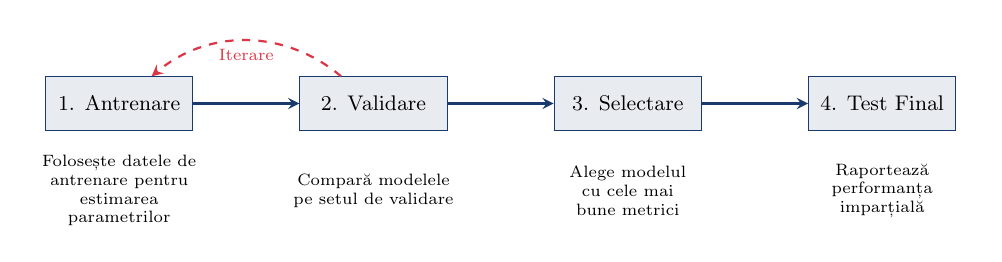
\begin{tikzpicture}[node distance=1.8cm, scale=0.85, transform shape]
        \tikzstyle{process} = [rectangle, minimum width=2.2cm, minimum height=0.8cm, text centered, draw=MainBlue, fill=MainBlue!10, font=\small]
        \tikzstyle{arrow} = [->, >=stealth, thick, MainBlue]

        % Nodes
        \node (train) [process] {1. Antrenare};
        \node (validate) [process, right of=train, xshift=2cm] {2. Validare};
        \node (select) [process, right of=validate, xshift=2cm] {3. Selectare};
        \node (test) [process, right of=select, xshift=2cm] {4. Test Final};

        % Arrows
        \draw [arrow] (train) -- (validate);
        \draw [arrow] (validate) -- (select);
        \draw [arrow] (select) -- (test);

        % Feedback loop
        \draw [arrow, dashed, Crimson] (validate) to[bend right=40] node[below, font=\scriptsize] {Iterare} (train);

        % Labels below
        \node [below of=train, yshift=0.5cm, font=\scriptsize, text width=2.5cm, align=center] {Folosește datele de\\antrenare pentru\\estimarea parametrilor};
        \node [below of=validate, yshift=0.5cm, font=\scriptsize, text width=2.5cm, align=center] {Compară modelele\\pe setul de validare};
        \node [below of=select, yshift=0.5cm, font=\scriptsize, text width=2.5cm, align=center] {Alege modelul\\cu cele mai bune metrici};
        \node [below of=test, yshift=0.5cm, font=\scriptsize, text width=2.5cm, align=center] {Raportează\\performanța imparțială};
    \end{tikzpicture}
    \end{center}

    \vspace{0.15cm}

    \begin{alertblock}{Regulă Critică}
        \textbf{Niciodată} nu folosiți setul de test pentru selecția modelului! Aceasta cauzează \textit{scurgere de date} și estimări prea optimiste ale performanței.
    \end{alertblock}
\end{frame}

\begin{frame}{Date Reale: Compararea Prognozelor}
    \begin{columns}[T]
        \column{0.32\textwidth}
        \begin{exampleblock}{Interpretare}
            Date pasageri companii aeriene: Holt-Winters Multiplicativă performează cel mai bine pentru date sezoniere.
        \end{exampleblock}
        \vspace{0.3cm}
        \quantlet{TSA\_ch0\_real\_data}{https://github.com/QuantLet/TSA/tree/main/TSA_ch0/TSA_ch0_real_data}
        \column{0.66\textwidth}
        \vspace{-0.3cm}
        \begin{center}
            \includegraphics[width=\textwidth, height=0.80\textheight, keepaspectratio]{real_data_forecast_comparison.pdf}
        \end{center}
    \end{columns}
\end{frame}

\begin{frame}{Performanța Prognozei pe Diferite Seturi de Date}
    \begin{columns}[T]
        \column{0.32\textwidth}
        \begin{exampleblock}{Interpretare}
            Serii diferite necesită modele diferite. Datele sezoniere necesită metode sezoniere.
        \end{exampleblock}
        \vspace{0.3cm}
        \quantlet{TSA\_ch0\_multi\_series}{https://github.com/QuantLet/TSA/tree/main/TSA_ch0/TSA_ch0_multi_series}
        \column{0.66\textwidth}
        \vspace{-0.3cm}
        \begin{center}
            \includegraphics[width=\textwidth, height=0.80\textheight, keepaspectratio]{multiple_series_comparison.pdf}
        \end{center}
    \end{columns}
\end{frame}

%=============================================================================
% SECȚIUNEA 5: MODELAREA SEZONALITĂȚII
%=============================================================================
\section{Modelarea Sezonalității}

\begin{frame}{Modelarea Sezonalității: Două Abordări}
    \begin{columns}[T]
        \begin{column}{0.48\textwidth}
            \textbf{1. Variabile Dummy:}

            \vspace{0.1cm}
            $X_t = \mu + \sum_{j=1}^{s-1}\gamma_j D_{jt} + \varepsilon_t$

            \vspace{0.2cm}
            \begin{itemize}
                \item $D_{jt} = 1$ dacă $t$ în sezonul $j$
                \item $s-1$ parametri
                \item Orice tipar sezonier
            \end{itemize}
        \end{column}
        \begin{column}{0.48\textwidth}
            \textbf{2. Termeni Fourier:}

            \vspace{0.1cm}
            $X_t = \mu + \sum_{k=1}^{K}[\alpha_k\sin(\cdot) + \beta_k\cos(\cdot)]$

            \vspace{0.2cm}
            \begin{itemize}
                \item Funcții sinusoidale
                \item $2K$ parametri
                \item Tipare netede
            \end{itemize}
        \end{column}
    \end{columns}

    \vspace{0.15cm}

    \begin{alertblock}{Compromis}
        \begin{itemize}
            \item \textbf{Dummy}: orice tipar, mai mulți parametri
            \item \textbf{Fourier}: netede, mai puțini parametri
        \end{itemize}
    \end{alertblock}
\end{frame}

\begin{frame}{Variabile Dummy vs Termeni Fourier}
    \begin{columns}[T]
        \column{0.35\textwidth}
        \begin{block}{Comparație}
            \begin{itemize}
                \item \textbf{Dummy}: captează orice formă dar necesită $s-1$ parametri
                \item \textbf{Fourier}: folosește $2K$ parametri pentru tipare netede
            \end{itemize}
        \end{block}
        \vspace{0.3cm}
        \quantlet{TSA\_ch0\_fourier}{https://github.com/QuantLet/TSA/tree/main/TSA_ch0/TSA_ch0_fourier}
        \column{0.63\textwidth}
        \vspace{-0.3cm}
        \begin{center}
            \includegraphics[width=\textwidth, height=0.78\textheight, keepaspectratio]{seasonality_fourier_dummies.pdf}
        \end{center}
    \end{columns}
\end{frame}

\begin{frame}{Alegerea între Dummy și Fourier}
    \begin{center}
    \small
    \begin{tabular}{lcc}
        \toprule
        \textbf{Criteriu} & \textbf{Dummy} & \textbf{Fourier} \\
        \midrule
        Parametri (lunar) & 11 & $2K$ (adesea 4--6) \\
        Tipar sezonier & Orice formă & Neted/sinusoidal \\
        Interpretare & Directă (efecte lunare) & Componente de frecvență \\
        Sezoane de înaltă frecvență & Mulți parametri & Eficient \\
        Sezonalitate multiplă & Complex & Ușor (adăugați termeni) \\
        \bottomrule
    \end{tabular}
    \end{center}

    \vspace{0.1cm}

    \begin{exampleblock}{Recomandări}
        \begin{itemize}
            \item Folosiți \textbf{dummy}: tipare neregulate, coeficienți interpretabili
            \item Folosiți \textbf{Fourier}: tipare netede, sezonalitate de înaltă frecvență, perioade multiple
            \item \textbf{Termenii Fourier} sunt folosiți în TBATS și Facebook Prophet
        \end{itemize}
    \end{exampleblock}
\end{frame}

%=============================================================================
% SECȚIUNEA 6: GESTIONAREA TRENDULUI ȘI SEZONALITĂȚII
%=============================================================================
\section{Gestionarea Trendului și Sezonalității}

\begin{frame}{De Ce Eliminăm Trendul și Sezonalitatea?}
    \textbf{Înainte de modelare}, adesea trebuie să facem seria staționară:

    \vspace{0.15cm}

    \begin{columns}[T]
        \begin{column}{0.48\textwidth}
            \textbf{Motive pentru detrendare:}
            \begin{itemize}
                \item Cerința de staționaritate
                \item Focus pe fluctuații
                \item Evitarea regresiei false
                \item Permiterea inferenței valide
            \end{itemize}
        \end{column}
        \begin{column}{0.48\textwidth}
            \textbf{Motive pentru desezonalizare:}
            \begin{itemize}
                \item Dezvăluirea trendului subiacent
                \item Comparații între sezoane
                \item Simplificarea modelării
                \item Focus pe componenta neregulată
            \end{itemize}
        \end{column}
    \end{columns}

    \vspace{0.2cm}

    \begin{alertblock}{Important}
        După modelarea seriei detrendate/desezonalizate, trebuie să \textbf{inversăm transformarea} pentru prognoză.
    \end{alertblock}
\end{frame}

\begin{frame}{Metode de Eliminare a Trendului}
    \begin{columns}[T]
        \column{0.55\textwidth}
        \begin{block}{Șase Abordări Comune de Detrendare}
            \begin{enumerate}
                \item \textbf{Diferențiere}: $\Delta X_t = X_t - X_{t-1}$
                \item \textbf{Regresie liniară}: $\hat{T}_t = \hat{\beta}_0 + \hat{\beta}_1 t$
                \item \textbf{Polinomială}: Polinom de ordin superior
                \item \textbf{Filtru HP}: Echilibru estimare vs netezime
                \item \textbf{Media mobilă}: $\hat{T}_t = MA_q(X_t)$
                \item \textbf{LOESS}: Regresie polinomială locală
            \end{enumerate}
        \end{block}
        \column{0.43\textwidth}
        \begin{exampleblock}{Alegerea Depinde De}
            \begin{itemize}
                \item Natura trendului (determinist vs stochastic)
                \item Scopul (prognoză vs analiză)
            \end{itemize}
        \end{exampleblock}
    \end{columns}
\end{frame}

\begin{frame}{Metode de Detrendare: Comparație}
    \begin{columns}[T]
        \column{0.32\textwidth}
        \begin{alertblock}{Idee Cheie}
            Metode diferite produc reziduuri diferite. Alegeți în funcție de tipul de trend și obiectivele analizei.
        \end{alertblock}
        \vspace{0.3cm}
        \quantlet{TSA\_ch0\_detrending}{https://github.com/QuantLet/TSA/tree/main/TSA_ch0/TSA_ch0_detrending}
        \column{0.66\textwidth}
        \vspace{-0.3cm}
        \begin{center}
            \includegraphics[width=\textwidth, height=0.80\textheight, keepaspectratio]{detrending_methods.pdf}
        \end{center}
    \end{columns}
\end{frame}

% Slide removed: "Estimarea Trendului: Abordări Multiple" — redundant with "Metode de Detrendare: Comparație" (slide 53)

\begin{frame}{Filtrul Hodrick-Prescott (HP)}
    \begin{defn}[Filtrul HP]
        \textbf{Filtrul HP} descompune $X_t$ în trend $\tau_t$ și ciclu $c_t$: $X_t = \tau_t + c_t$, prin minimizarea:
        \vspace{-0.2cm}
        {\small\[
            \min_{\{\tau_t\}} \left\{ \sum_{t=1}^{T}(X_t - \tau_t)^2 + \lambda \sum_{t=2}^{T-1}[(\tau_{t+1} - \tau_t) - (\tau_t - \tau_{t-1})]^2 \right\}
        \]}
        \vspace{-0.3cm}
    \end{defn}

    \begin{columns}[T]
        \column{0.48\textwidth}
        \begin{block}{Interpretare}
            \begin{itemize}
                \item Primul termen: ajustare la date
                \item Al doilea termen: penalizare netezime
                \item $\lambda$: parametru de compromis
            \end{itemize}
        \end{block}
        \column{0.5\textwidth}
        \begin{exampleblock}{Valori Standard $\lambda$}
            \begin{itemize}
                \item Anual: $\lambda = 6.25$
                \item Trimestrial: $\lambda = 1600$
                \item Lunar: $\lambda = 129600$
            \end{itemize}
        \end{exampleblock}
    \end{columns}
\end{frame}

\begin{frame}{Filtrul HP: Efectul lui $\lambda$}
    \begin{center}
        \includegraphics[width=0.95\textwidth, height=0.52\textheight, keepaspectratio]{ch1_hp_filter_lambda.png}
    \end{center}
    \vspace{-0.2cm}
    \begin{block}{Compromis}
        \begin{itemize}
            \item \textbf{$\lambda$ mic}: Trendul urmează datele îndeaproape (mai flexibil)
            \item \textbf{$\lambda$ mare}: Trendul devine mai neted (se apropie de trend liniar)
        \end{itemize}
    \end{block}
    \quantlet{TSA\_ch1\_hp\_filter}{https://github.com/QuantLet/TSA/tree/main/TSA_ch1/TSA_ch1_hp_filter}
\end{frame}

\begin{frame}{Filtrul HP: Extragerea Ciclului de Afaceri}
    \begin{center}
        \includegraphics[width=0.95\textwidth, height=0.48\textheight, keepaspectratio]{ch1_hp_filter_cycle.png}
    \end{center}
    \vspace{-0.2cm}
    \begin{exampleblock}{Aplicație}
        Filtrul HP este utilizat pe scară largă în macroeconomie pentru extragerea ciclurilor de afaceri din PIB și alte serii economice.
    \end{exampleblock}
    \quantlet{TSA\_ch0\_hp\_cycle}{https://github.com/QuantLet/TSA/tree/main/TSA_ch0/TSA_ch0_hp_cycle}
\end{frame}

\begin{frame}{Filtrul HP: Limitări}
    \begin{columns}[T]
        \column{0.48\textwidth}
        \begin{alertblock}{Probleme Cunoscute}
            \begin{itemize}
                \item \textbf{Problema capetelor}: Estimările trendului nesigure la capete
                \item \textbf{Cicluri false}: Poate crea dinamici artificiale
                \item \textbf{Alegerea $\lambda$}: Rezultatele sensibile la parametru
                \item \textbf{Non-staționar}: Presupune că trendul este neted
            \end{itemize}
        \end{alertblock}
        \column{0.5\textwidth}
        \begin{exampleblock}{Alternative}
            \begin{itemize}
                \item \textbf{Filtre bandă}: Baxter-King, Christiano-Fitzgerald
                \item \textbf{Filtrul Hamilton}: Bazat pe regresie
                \item \textbf{Componente neobservate}: Modele space-state
            \end{itemize}
        \end{exampleblock}
    \end{columns}

    \vspace{0.2cm}

    \begin{block}{Critica lui Hamilton (2018)}
        ``De Ce Nu Ar Trebui Să Folosiți Niciodată Filtrul Hodrick-Prescott'' --- sugerează utilizarea regresiei pe valori întârziate în schimb.
    \end{block}
\end{frame}

\begin{frame}{Metode de Eliminare a Sezonalității}
    \begin{block}{Patru Abordări pentru Eliminarea Sezonalității}
        \begin{enumerate}
            \item \textbf{Diferențiere sezonieră}: $\Delta_s X_t = X_t - X_{t-s}$
            \item \textbf{Împărțire} (multiplicativ): $X_t^{adj} = X_t / \hat{S}_t$
            \item \textbf{Scădere} (aditiv): $X_t^{adj} = X_t - \hat{S}_t$
            \item \textbf{X-13ARIMA-SEATS}: Metodă statistică guvernamentală
        \end{enumerate}
    \end{block}

    \vspace{0.1cm}

    \begin{exampleblock}{Perioada Sezonieră $s$}
        \begin{itemize}
            \item Lunar $\Rightarrow s=12$
            \item Trimestrial $\Rightarrow s=4$
        \end{itemize}
    \end{exampleblock}
\end{frame}

\begin{frame}{Ajustare Sezonieră: Vizualizare}
    \begin{columns}[T]
        \column{0.32\textwidth}
        \begin{block}{Rezultat}
            Seria ajustată sezonier dezvăluie trendul subiacent fără fluctuațiile periodice.
        \end{block}
        \vspace{0.3cm}
        \quantlet{TSA\_ch0\_seasonal\_adj}{https://github.com/QuantLet/TSA/tree/main/TSA_ch0/TSA_ch0_seasonal_adj}
        \column{0.66\textwidth}
        \vspace{-0.3cm}
        \begin{center}
            \includegraphics[width=\textwidth, height=0.80\textheight, keepaspectratio]{seasonal_adjustment.pdf}
        \end{center}
    \end{columns}
\end{frame}

\begin{frame}{Trend Determinist vs Stochastic}
    \begin{columns}[T]
        \begin{column}{0.48\textwidth}
            \textbf{Trend Determinist:}
            \[
                X_t = \beta_0 + \beta_1 t + \varepsilon_t
            \]
            \begin{itemize}
                \item Trendul este o funcție de timp
                \item Detrendare prin regresie
                \item $\varepsilon_t$ este staționar
            \end{itemize}
        \end{column}
        \begin{column}{0.48\textwidth}
            \textbf{Trend Stochastic:}
            \[
                X_t = X_{t-1} + \varepsilon_t
            \]
            \begin{itemize}
                \item Componentă de mers aleatoriu
                \item Detrendare prin diferențiere
                \item $\Delta X_t$ este staționar
            \end{itemize}
        \end{column}
    \end{columns}

    \vspace{0.15cm}

    \begin{alertblock}{Metodă Greșită = Probleme}
        \begin{itemize}
            \item Diferențierea trendului determinist $\Rightarrow$ supra-diferențiere
            \item Regresie pe trend stochastic $\Rightarrow$ regresie falsă
        \end{itemize}
    \end{alertblock}
    \vspace{0.1cm}
    \begin{center}
        \includegraphics[width=0.85\textwidth, height=0.25\textheight, keepaspectratio]{trend_comparison_sidebyside.pdf}
    \end{center}
\end{frame}

\begin{frame}{Exemplu: Trend Determinist}
    \begin{columns}[T]
        \column{0.32\textwidth}
        \begin{exampleblock}{Cheie}
            Folosiți \textcolor{Crimson}{regresie} pentru eliminarea trendului $\succ$ reziduurile sunt staționare (ACF scade rapid).
        \end{exampleblock}
        \vspace{0.3cm}
        \quantlet{TSA\_ch0\_det\_trend}{https://github.com/QuantLet/TSA/tree/main/TSA_ch0/TSA_ch0_det_trend}
        \column{0.66\textwidth}
        \vspace{-0.3cm}
        \begin{center}
            \includegraphics[width=\textwidth, height=0.80\textheight, keepaspectratio]{deterministic_trend_example.pdf}
        \end{center}
    \end{columns}
\end{frame}

\begin{frame}{Exemplu: Trend Stochastic (Mers Aleatoriu)}
    \begin{columns}[T]
        \column{0.32\textwidth}
        \begin{exampleblock}{Cheie}
            Folosiți \textcolor{Crimson}{diferențiere} pentru eliminarea trendului $\succ$ diferențele sunt staționare (zgomot alb).
        \end{exampleblock}
        \vspace{0.3cm}
        \quantlet{TSA\_ch0\_stoch\_trend}{https://github.com/QuantLet/TSA/tree/main/TSA_ch0/TSA_ch0_stoch_trend}
        \column{0.66\textwidth}
        \vspace{-0.3cm}
        \begin{center}
            \includegraphics[width=\textwidth, height=0.80\textheight, keepaspectratio]{stochastic_trend_example.pdf}
        \end{center}
    \end{columns}
\end{frame}

% Slide removed: "Comparație Alăturată" — merged into "Trend Determinist vs Stochastic" (slide 63)

%=============================================================================
\section{Rezumat și Quiz}
%=============================================================================

\begin{frame}{Rezumat}
    \begin{block}{Ce Am Învățat}
        \begin{itemize}\setlength{\itemsep}{3pt}
            \item \textbf{Definiția Seriei de Timp}: Secvență de observații indexate după timp
            \item \textbf{Descompunere}: Componente Trend-Ciclu + Sezonier + Reziduu
            \item \textbf{Netezire Exponențială}: SES, Holt, Holt-Winters, cadrul ETS
            \item \textbf{Evaluarea Prognozei}: MAE, RMSE, MAPE; separări train/validare/test
        \end{itemize}
    \end{block}
    \vspace{0.2cm}
    \begin{exampleblock}{Idee Cheie}
        \begin{itemize}
            \item \textbf{Înțelegeți Înainte de a Modela}:
            \begin{itemize}
                \item Întotdeauna vizualizați și descompuneți datele mai întâi
                \item Alegeți aditiv vs multiplicativ în funcție de comportamentul varianței
            \end{itemize}
        \end{itemize}
    \end{exampleblock}
\end{frame}

\begin{frame}{Quiz Rapid}
    \begin{center}
    \begin{minipage}{0.9\textwidth}
    \begin{enumerate}\setlength{\itemsep}{10pt}
        \item[\textcolor{MainBlue}{\textbf{1.}}] Care este diferența între descompunerea aditivă și multiplicativă?
        \item[\textcolor{MainBlue}{\textbf{2.}}] Când ar trebui să folosiți Holt-Winters în loc de netezire exponențială simplă?
        \item[\textcolor{MainBlue}{\textbf{3.}}] De ce nu putem folosi validare încrucișată standard k-fold pentru serii de timp?
        \item[\textcolor{MainBlue}{\textbf{4.}}] Ce înseamnă $\alpha = 0.9$ în netezirea exponențială?
        \item[\textcolor{MainBlue}{\textbf{5.}}] Cum distingeți între trend determinist și stochastic?
    \end{enumerate}
    \end{minipage}
    \end{center}
\end{frame}

\begin{frame}{Răspunsuri Quiz}
    \begin{center}
    \begin{minipage}{0.9\textwidth}
    {\small
    \begin{enumerate}
        \item[\textcolor{MainBlue}{\textbf{1.}}] \textbf{Aditivă vs Multiplicativă}: Aditivă când amplitudinea sezonieră este constantă; multiplicativă când crește odată cu nivelul.
        \vspace{0.1cm}
        \item[\textcolor{MainBlue}{\textbf{2.}}] \textbf{Holt-Winters}: Când datele au atât trend CÂT ȘI sezonalitate. SES gestionează doar nivelul.
        \vspace{0.1cm}
        \item[\textcolor{MainBlue}{\textbf{3.}}] \textbf{CV Serii de Timp}: K-fold standard ignoră ordinea temporală --- ar folosi date viitoare pentru a prezice trecutul (scurgere de date).
        \vspace{0.1cm}
        \item[\textcolor{MainBlue}{\textbf{4.}}] \textbf{$\alpha = 0.9$}: Pondere mare pe observațiile recente, prognoza reacționează rapid la schimbări dar este mai volatilă.
        \vspace{0.1cm}
        \item[\textcolor{MainBlue}{\textbf{5.}}] \textbf{Tipul de trend}: Determinist --- funcție predictibilă de timp (folosiți regresie). Stochastic --- componentă de mers aleatoriu (folosiți diferențiere).
    \end{enumerate}
    }
    \end{minipage}
    \end{center}
\end{frame}

\begin{frame}{Ce Urmează?}
    \begin{center}
    \begin{minipage}{0.85\textwidth}
    \begin{block}{Capitolul 1: Procese Stochastice și Staționaritate}
        \begin{itemize}
            \item \textbf{Procese Stochastice}: Fundament matematic pentru serii de timp
            \begin{itemize}
                \item Variabile aleatoare indexate după timp
                \item Staționaritate strictă vs slabă (covarianță)
            \end{itemize}
            \item \textbf{Procese Cheie}: Zgomot alb și mers aleatoriu
            \begin{itemize}
                \item Blocuri de construcție pentru modelele ARIMA
                \item Înțelegerea revertirii la medie vs rădăcini unitare
            \end{itemize}
            \item \textbf{ACF și PACF}: Instrumente pentru identificarea modelului
            \begin{itemize}
                \item Detectarea structurii de autocorelație
                \item Alegerea ordinelor AR și MA
            \end{itemize}
        \end{itemize}
    \end{block}
    \end{minipage}
    \end{center}

    \begin{center}
        \Large\textcolor{MainBlue}{Întrebări?}
    \end{center}
\end{frame}

%=============================================================================
% BIBLIOGRAFIE
%=============================================================================
\section{Bibliografie}

\begin{frame}{Bibliografie I}
    \vspace{-0.3cm}
    \begin{cminipage}{0.95\textwidth}
    \begin{block}{Lucrări fundamentale}
        {\small
        \begin{itemize}\setlength{\itemsep}{0pt}
            \item Holt, C.C. (1957). Forecasting Seasonals and Trends by Exponentially Weighted Moving Averages, ONR Research Memorandum No. 52.
            \item Winters, P.R. (1960). Forecasting Sales by Exponentially Weighted Moving Averages, \textit{Management Science}, 6(3), 324--342.
            \item Cleveland, R.B., Cleveland, W.S., McRae, J.E., \& Terpenning, I. (1990). STL: A Seasonal-Trend Decomposition, \textit{Journal of Official Statistics}, 6(1), 3--73.
            \item Hodrick, R.J., \& Prescott, E.C. (1997). Postwar U.S. Business Cycles: An Empirical Investigation, \textit{Journal of Money, Credit and Banking}, 29(1), 1--16.
        \end{itemize}
        }
    \end{block}

    \begin{exampleblock}{Manuale clasice}
        {\small
        \begin{itemize}\setlength{\itemsep}{0pt}
            \item Hamilton, J.D. (1994). \textit{Time Series Analysis}, Princeton University Press.
            \item Brockwell, P.J., \& Davis, R.A. (2016). \textit{Introduction to Time Series and Forecasting}, 3rd ed., Springer.
            \item Shumway, R.H., \& Stoffer, D.S. (2017). \textit{Time Series Analysis and Its Applications}, 4th ed., Springer.
        \end{itemize}
        }
    \end{exampleblock}
    \end{cminipage}
\end{frame}

\begin{frame}{Bibliografie II}
    \begin{cminipage}{0.95\textwidth}
    \begin{block}{Referințe moderne}
        {\small
        \begin{itemize}\setlength{\itemsep}{0pt}
            \item Hyndman, R.J., \& Athanasopoulos, G. (2021). \textit{Forecasting: Principles and Practice}, 3rd ed., OTexts.
            \item Hyndman, R.J., Koehler, A.B., Ord, J.K., \& Snyder, R.D. (2008). \textit{Forecasting with Exponential Smoothing: The State Space Approach}, Springer.
            \item Gardner, E.S. (2006). Exponential Smoothing: The State of the Art -- Part II, \textit{International Journal of Forecasting}, 22(4), 637--666.
        \end{itemize}
        }
    \end{block}

    \begin{exampleblock}{Resurse online și cod}
        {\small
        \begin{itemize}\setlength{\itemsep}{0pt}
            \item \textbf{Quantlet}: \url{https://quantlet.com} $\succ$ Platformă de cod pentru metode cantitative
            \item \textbf{Quantinar}: \url{https://quantinar.com} $\succ$ Platformă de învățare pentru metode cantitative
            \item \textbf{GitHub TSA}: \url{https://github.com/QuantLet/TSA/tree/main/TSA_ch0} $\succ$ Cod Python pentru acest capitol
        \end{itemize}
        }
    \end{exampleblock}
    \end{cminipage}
\end{frame}

\begin{frame}{}
    \begin{cminipage}{0.95\textwidth}
    \centering
    \vspace{1cm}

    \Huge\textcolor{MainBlue}{Vă Mulțumim!}

    \vspace{0.8cm}

    \Large Întrebări?

    \vspace{1cm}

    {\normalsize
    \textcolor{MediumGray}{Prof. dr. Daniel Traian Pele}\\[0.2cm]
    \textcolor{MediumGray}{\texttt{danpele@ase.ro}}\\[0.3cm]
    \href{https://github.com/QuantLet/TSA}{\textcolor{MainBlue}{github.com/QuantLet/TSA}}
    }

    \vspace{0.5cm}
    \end{cminipage}
\end{frame}

\end{document}
